% A good introduction to latex can be found here:
%  http://www.cse.ohio-state.edu/~hank/latex/lshort141.pdf

\documentclass{article}

\usepackage{full page}  % make the margins somewhat smaller than the default

\usepackage{listings}  %  needed for source code listings
\usepackage{color}
\usepackage{graphicx}

\definecolor{javared}{rgb}{0.6,0,0} % for strings
\definecolor{javagreen}{rgb}{0.25,0.5,0.35} % comments
\definecolor{javapurple}{rgb}{0.5,0,0.35} % keywords
\definecolor{javadocblue}{rgb}{0.25,0.35,0.75} % javadoc
 
\lstset{language=Java,
basicstyle=\ttfamily,
keywordstyle=\color{javapurple}\bfseries,
stringstyle=\color{javared},
commentstyle=\color{javagreen},
morecomment=[s][\color{javadocblue}]{/**}{*/},
numbers=left,
numberstyle=\tiny\color{black},
stepnumber=2,
numbersep=10pt,
tabsize=4,
showspaces=false,
showstringspaces=false} 

% set the document title, author, and date here.
%  once set, the \maketitle command (within the document)
%  will display them nicely
\title{Missionaries and Cannibals Solution}
\author{Junjie Guan}

\begin{document}
\maketitle

\section{Introduction}
We can convert each state of carnibal problem into one code, by using factoring. The only three factors that relate to the state are the numbers of minssionary, carnibals and boats. Assuming there is a the range of the number is $R$, the formula can be described as followed:
$$v = n_m \times R^2 + n_c \times R^1 + n_b \times R^0$$
where the $v$ represents tha encoded value, $n_m, n_c, n_b$ represent the number of missionary, carnibal and boats respectively. Let's say $R = 10$, and the initial state of the problem are $n_m = 3, n_c = 3, n_b = 1$, I can use a graph to describe the relationship between different states (for simplicity, I only the major parts of the graph).

\begin{figure*}[!h]
\centering
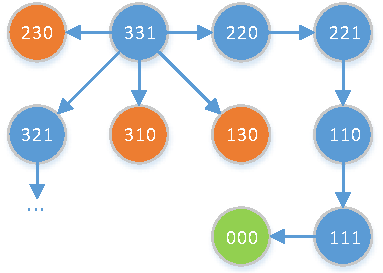
\includegraphics[width=0.5\textwidth]{hw1.pdf}
\caption{A sample graph of states that describe carnibal problem starting with (3, 3, 1), the blue nodes are the normal states, green is the final state, and the orange ones are illegal states.}
\label{states}
\end{figure*}

In Figure \ref{states}, we can see that from a starting states, differnet actions lead to different path, some of them will eventually go to the goal, some of them will run into a dead end.

\section{Implementation of the model}
Now you are ready to write and test the code that implements the model. (You'll write the search algorithms in the next section.) CannibalProblem.java is your starting point. Ultimately, this will extend 'UUSearchProblem', but for now, UUSearchProblem is unfinished and thus broken, so you probably want to delete the 'extends' keyword.
A CannibalProblem instance should keep track of how many cannibals and missionaries there are in the problem (three of each is standard, but your solution should be general).

The CannibalProblem class is also a good place to put an inner class that represents nodes for the search. A CannibalNode will represent the "current" state of the problem at some point in the exploration. For example, at some point in the search, we might be exploring the (2, 2, 1) state.

A 'CannibalNode' should provide a method that creates a list of nodes that represent legal states reachable using legal actions from the current node. I called this getSuccessors, but you'll have ot implement the body of the method. Also implement any other methods that have a comment like "you write this" in the provided code.

Test your code thoroughly before you go on; write some test code (perhaps in a main method of CannibalProblem) that creates some nodes, finds their successors, and prints out the results. The results should agree with those that you drew for the intro. This testing step is not only required, but important. Errors in your model will lead to very-hard to diagnose errors that will make it virtually impossible to debug your search algorithms.

Present the work in your report. Include the key parts of your code using the listings environment in LaTeX, and discuss how the code works. Also describe your testing and convince the reader that your testing process demonstrated correctness of your code.



The model is implemented in 
\verb`CannibalProblem.java`.  Here's my code for \verb`getSuccessors`:

\begin{lstlisting}[numbers=left]
public ArrayList<UUSearchNode> getSuccessors() {
  ArrayList<UUSearchNode> successors = new ArrayList<>();
  if (state[2] != 0) {
    // search from the possible largest number
    for (int i = 0; i <= Math.min(state[2] * BOAT_SIZE, state[0]); i++) {
      for (int j = 0; j <= Math.min(state[2] * BOAT_SIZE - i,
          state[1]); j++) {
        if(i + j == 0) continue;
        CannibalNode tryNode = new CannibalNode(state[0] - i,
            state[1] - j, 0, 0);
        if (isSafeState(tryNode)) {
          successors.add(tryNode);
        }
      }
    }
  } else {
    CannibalNode tryNode = new CannibalNode(state[0], state[1],
        totalBoats, 0);
    successors.add(tryNode);
  }
  return successors;
}
\end{lstlisting}

The basic idea of \verb`getSuccessors` is to traverse through every possible state that is contraint by the problem defination (such as number of missionary and carnibals, the size of the boat). After getting a new state, it immediately checkes if it is legal. Finally it put the state node into successors list if it is safe.

The order of getting successors is vital to depth first search. I did optimize the codes for DFS, so that during each action it can go to the optimal state, which is transmitting as much people as possible. Simply by replacing line 6-7 to :

\begin{lstlisting}[numbers=left]
for (int i = Math.min(state[2] * BOAT_SIZE, state[0]); i >= 0 ; i--) {
  for (int j = Math.min(state[2] * BOAT_SIZE - i,
    state[1]); j >= 0; j--) {
\end{lstlisting}
However, this will lose a lot fun, because by doing so there are almost no difference between different search algorithm. So latter I stick to the non-optimized one.

I used a method \verb`isSafeState` that returns \verb`true` if the state is legal. Basically it checks the legal state of both side of the river. Here are the codes.

\begin{lstlisting}[numbers=left]
private boolean isSafeState(CannibalNode tryNode) {
  if (tryNode.state[0] >= tryNode.state[1]
      && (totalMissionaries - tryNode.state[0]) 
        >= (totalCannibals - tryNode.state[1])
      && tryNode.state[0] >= 0 && tryNode.state[1] >= 0)
    return true;
  else
    return false;
}
\end{lstlisting}

\section{Breadth-first search}


\begin{lstlisting}[numbers=left][language=Java]
  public List<UUSearchNode> breadthFirstSearch() {
    resetStats();

    UUSearchNode node = startNode;
    HashMap<UUSearchNode, UUSearchNode> visited = new HashMap<>();
    Queue<UUSearchNode> nqueue = new LinkedList<UUSearchNode>();
    List<UUSearchNode> successors;

    nqueue.add(startNode);
    while (!nqueue.isEmpty()) {
      // get node from the queue
      node = nqueue.poll();

      // check if arrives destination
      if (node.goalTest()) {
        updateMemory(visited.size() + 1); // add the start node
        nodesExplored = visited.size() + 1;
        return backchain(node, visited);
      }

      // if not destination, keep searching and tracking
      successors = node.getSuccessors();
      for (UUSearchNode n : successors) {

        if (!visited.containsValue(n)) {
          visited.put(n, node);
          nqueue.add(n);
        }
      }
    }
    // if destination not found, return null
    return null;
  }
\end{lstlisting}

\begin{lstlisting}[numbers=left]
bfs path length:  6 [0, 111, 110, 221, 220, 331]
Nodes explored during last search:  6
Maximum memory usage during last search 6
Total execution time: 0.7 seconds
\end{lstlisting}




\section{Memoizing depth-first search}

\begin{lstlisting}[numbers=left]
public List<UUSearchNode> depthFirstMemoizingSearch(int maxDepth) {
  resetStats();
  HashMap<UUSearchNode, Integer> visited = new HashMap<>();
  return dfsrm(startNode, visited, 0, maxDepth);
}

private List<UUSearchNode> dfsrm(UUSearchNode currentNode,
    HashMap<UUSearchNode, Integer> visited, int depth, int maxDepth) {

  // keep track of stats; these calls charge for the current node
  updateMemory(visited.size());
  incrementNodeCount();

  // you write this method. Comments *must* clearly show the
  // "base case" and "recursive case" that any recursive function has.

  //System.out.println(currentNode);
  List<UUSearchNode> tryPath, path = new ArrayList<UUSearchNode>(
      Arrays.asList(currentNode));
  List<UUSearchNode> successors;

  visited.put(currentNode, 1);
  if (depth > maxDepth)
    return null;      
  
  if (currentNode.goalTest()) {
    return path;
  } else {
    successors = currentNode.getSuccessors();
    for (UUSearchNode n : successors) {
      if (!visited.containsKey(n)) {
        //System.out.println(visited.size());
        tryPath = dfsrm(n, visited, depth + 1, maxDepth);
        if (tryPath != null) {
          path.addAll(tryPath);
          return path;
        }
      }
    }
  }
  return null;
}
\end{lstlisting}

\section{Path-checking depth-first search}

\begin{lstlisting}[numbers=left]
public List<UUSearchNode> depthFirstPathCheckingSearch(int maxDepth) {
  resetStats();
  HashSet<UUSearchNode> currentPath = new HashSet<UUSearchNode>();
  return dfsrpc(startNode, currentPath, 0, maxDepth);
}

private List<UUSearchNode> dfsrpc(UUSearchNode currentNode,
    HashSet<UUSearchNode> currentPath, int depth, int maxDepth) {

  // keep track of stats; these calls charge for the current node
  updateMemory(currentPath.size());
  incrementNodeCount();

  List<UUSearchNode> successors, tryPath, path = new ArrayList<UUSearchNode>(
      Arrays.asList(currentNode));

  //System.out.println(currentNode);
  if (depth > maxDepth)
    return null;
  else 
    currentPath.add(currentNode);

  // This is base case where search reaches the goal
  if (currentNode.goalTest()) {
    return path;
  } else {
  
    successors = currentNode.getSuccessors();
    for (UUSearchNode n : successors) {
      if (!currentPath.contains(n)) {
        // This is the recursive function
        tryPath = dfsrpc(n, currentPath, depth + 1, maxDepth);
        if (tryPath != null) {
          path.addAll(tryPath);
          return path;
        }
      }
    }
  }
  currentPath.remove(currentNode);
  return null;
}
\end{lstlisting}

\section{Iterative deepening search}

\begin{lstlisting}[numbers=left]
public List<UUSearchNode> IDSearch(int maxDepth) {
  resetStats();
  HashSet<UUSearchNode> currentPath = new HashSet<UUSearchNode>();
  List<UUSearchNode> path;
  for (int i = 1; i <= maxDepth; i++) {
    currentPath.clear();
    path = dfsrpc(startNode, currentPath, 0, i);
    if (path != null)
      return path;
  }
  return null;
}
\end{lstlisting}

\section{Lossy missionaries and cannibals}

\end{document}